% =====================================================================
% Epoch-Dependent Acceleration Scale from Bounded Topology:
%   Predictions for High-Redshift Galactic Dynamics
%
% B. Shatto (Independent Researcher)
% ORCID iD: 0009-0007-4419-1311
%
% Source converted from a0-evolution-paper.md (lean PRD draft).
% Figures live in figures/figure{1..4}.pdf alongside this file.
% Bibliography is inline (thebibliography environment); no separate .bib.
%
% Compile with pdflatex (two passes for cross-references):
%   pdflatex a0z-paper && pdflatex a0z-paper
% =====================================================================

\documentclass[
    aps,
    prd,
    reprint,
    superscriptaddress,
    nofootinbib,
    floatfix
]{revtex4-2}

\usepackage[utf8]{inputenc}
\usepackage{amsmath}
\usepackage{amssymb}
\usepackage{graphicx}
\usepackage{booktabs}
\usepackage{enumitem}
\usepackage{xspace}
\usepackage{xcolor}
\usepackage{hyperref}

% Modest colored hyperlinks for PDF; revtex4-2 loads hyperref so we only
% tune the link colors here.
\hypersetup{
    colorlinks=true,
    linkcolor=blue!50!black,
    citecolor=blue!50!black,
    urlcolor=blue!70!black,
}

% Hyphenation hints (lowercase only -- TeX forbids uppercase / digits)
\hyphenation{bary-onic mono-tonic strat-i-fied iso-tropy
             cos-mo-log-i-cal eigen-value}

\begin{document}

\title{Epoch-Dependent Acceleration Scale from Bounded Topology:
       Predictions for High-Redshift Galactic Dynamics}

\author{B.~Shatto}
\thanks{ORCID iD: \href{https://orcid.org/0009-0007-4419-1311}{0009-0007-4419-1311}}
\email{bshatto.pe@gmail.com}
\affiliation{Independent Researcher, St.~Petersburg, Florida, USA}

\date{\today}

\begin{abstract}
The MOND acceleration scale $a_0 \approx 1.20 \times 10^{-10}$~m/s$^2$
satisfies $a_0/(cH_0) \approx 0.18$, a coincidence unexplained for four
decades. Within a bounded-topology measurement framework on
$S^1 = \partial(\text{M\"obius}) \hookrightarrow S^3$
(Appendix~\ref{app:framework}), separately calibrated assignments of
$a_0$ and $H$ to specific phase positions on the 120-domain of $S^3/2I$
produce this ratio as an algebraic consequence of the shared edge-mode
hierarchy, with the non-trivial content carried by the 0.7\% match at a
combinatorially sparse position: $C(13/120)/C(34/120) = 0.1845$,
agreeing with the observed $0.1833$ at $0.7\%$ and unique among the
framework's Fibonacci-well pairs. Because both observables reference the
same epoch-dependent hierarchy, the ratio holds at every redshift:
$a_0(z) = a_0(0)\,E(z)$. Five observable channels follow as powers of
$E(z)$ with no additional free parameter: the baryonic Tully-Fisher
normalization ($E^{-1}$), the MOND transition radius ($E^{-1/2}$), the
asymptotic velocity at fixed baryonic mass ($E^{+1/4}$), the
Newtonian-inferred lensing enhancement ($E^{+1/2}$), and the
gravitational collapse time ($E^{-1/4}$). The lensing channel predicts
a mass- and aperture-universal 74\% enhancement of $M_\text{dyn}/M_b$
at $z = 2$, testable through mass- and aperture-stratified Euclid DR1
stacking in October 2026 and distinct from the mass- and
aperture-dependent $\Lambda$CDM halo-concentration alternative. The
same selection rule leaves $\Lambda$ fixed, separating the evolving
galactic scale from the dark-energy sector. Existing constraints
include a provisional 2.9$\sigma$ trend-shape tension with the KMOS3D
Tully-Fisher data, tested by forward modeling and not dissolved.
\end{abstract}

\maketitle

% =====================================================================
\section{Introduction}
\label{sec:intro}
% =====================================================================

The MOND acceleration scale $a_0 \approx 1.20 \times 10^{-10}$~m/s$^2$
has governed the phenomenology of galactic rotation curves for four
decades~\cite{Milgrom1983}. Fitted to the local SPARC sample with
intrinsic scatter of 0.1 dex~\cite{Lelli2016, Famaey2012}, it satisfies
a numerical coincidence that has never been explained:
$a_0/(cH_0) \approx 0.18$, with the Hubble rate setting the dimensional
scale of the MOND threshold~\cite{Milgrom1999, McGaugh2004}. Within
standard MOND this ratio is an accident. Within $\Lambda$CDM it has no
physical content. It has remained unexplained since Milgrom first noted
it in 1983.

Three current observational tensions share this same dimensional anchor.

First, the coincidence itself. Using the standard SPARC
normalization~\cite{Lelli2016} and Planck background
value~\cite{Planck2018}, $a_0/(cH_0) = 0.183$, numerically stable
across four decades of improving measurements with no theoretical
account of why.

Second, JWST has revealed candidate galaxies at $z \sim 7\text{--}10$
with stellar masses $M_\star \gtrsim 10^{10}\,M_\odot$ assembled within
600 Myr of the Big Bang~\cite{Labbe2023, BoylanKolchin2023}. Under
standard halo-growth assumptions, the most extreme candidates imply
unusually high star-formation efficiencies and have been discussed as a
potential early-structure tension. If $a_0$ were larger at early times,
gravitational collapse would proceed faster and the tension would ease.

Third, DESI DR2, combined with CMB and supernova data, strengthens the
reported preference for an evolving dark-energy equation of
state~\cite{DESI2025}. If $\Lambda$ is actually constant and the
apparent evolution is a template artifact, the question becomes what
\emph{does} evolve with the Hubble rate. The framework explored here
answers: $a_0$.

This paper develops one hypothesis and its consequences. Within a
bounded-topology measurement framework on
$S^1 = \partial(\text{M\"obius}) \hookrightarrow S^3$
(Appendix~\ref{app:framework}), the Milgrom ratio resolves to the ratio
of two phase-operator values at adjacent Fibonacci wells on the
120-domain native to $S^3/2I$:
\begin{equation}
\frac{a_0}{cH} = \frac{C(13/120)}{C(34/120)} = 0.1845,
\label{eq:milgrom-ratio}
\end{equation}
agreeing with the observed $0.1833$ at the $0.7\%$ level. The ratio
itself is not a separate adjustable parameter: once the $a_0$ and $H$
wells are fixed by separately calibrated well assignments sharing the
same edge-mode hierarchy, Eq.~(\ref{eq:milgrom-ratio}) follows
algebraically. The non-trivial content is the 0.7\% match at a
combinatorially sparse position (Sec.~\ref{sec:derivation}). Among the
framework's six Fibonacci-well pairs, $(13, 34)$ is the unique pair
that reproduces the observed ratio within 1\%
(Sec.~\ref{sec:derivation}).

Because both $a_0$ and $H$ reference the same epoch-dependent
hierarchy in the framework's scaling law, the ratio
Eq.~(\ref{eq:milgrom-ratio}) holds at every cosmic epoch. The evolution
follows:
\begin{equation}
a_0(z) = a_0(0)\,E(z), \qquad E(z) \equiv H(z)/H_0.
\label{eq:a0-evolution}
\end{equation}

The bare possibility $a_0 \propto H$ has appeared previously in
MOND-motivated discussions of the Milgrom coincidence. The novelty
here is not the dimensional guess, but the specific framework
mechanism: the ratio is fixed by $C(13/120)/C(34/120)$, the evolution
is linear in $E(z)$, and the five observable exponents are locked
together rather than tuned independently.

Five testable predictions follow as different powers of $E(z)$, with
no additional free parameter beyond the local SPARC calibration. The
Euclid DR1 release in October 2026 will deliver the sharpest test
through stacked galaxy-galaxy weak lensing at $z = 0.5\text{--}2$. The
framework's monotonic BTFR prediction is currently in tension with the
only existing intermediate-redshift measurement~\cite{Ubler2017}; this
tension is quantified in Sec.~\ref{sec:constraints} and held without
retreat.

Section~\ref{sec:derivation} derives Eqs.~(\ref{eq:milgrom-ratio}) and
(\ref{eq:a0-evolution}). Section~\ref{sec:channels} propagates the
evolution into five observable channels.
Section~\ref{sec:constraints} treats existing constraints.
Section~\ref{sec:euclid} specifies the Euclid test.
Section~\ref{sec:conclusions} closes.

% =====================================================================
\section{Derivation}
\label{sec:derivation}
% =====================================================================

The framework's measurement postulate (Appendix~\ref{app:framework})
maps any Planck-normalized observable to a phase position on the
120-domain native to $S^3/2I$:
\begin{equation}
\frac{A}{A_P} = C(\Theta) \cdot N^n,
\qquad C(\Theta) = 2\sin^2(\pi\Theta),
\label{eq:scaling-law}
\end{equation}
where $\Theta \in \{k/120\}$ is the phase position, $n$ the
manifold-mode index set by the embedding hierarchy
$S^1 \subset \text{M\"obius} \subset S^3$, and $N$ a dimensionless
hierarchy normalization that takes the form $(\sqrt{\Omega})^{-1}$
within each mode class, with its exact value fixed by calibrating one
reference observable per sector. The phase operator $C(\Theta)$ is
the squared ground-mode intensity on the M\"obius surface under
anti-periodic boundary conditions
(Appendix~\ref{app:framework-domain}). A selection rule assigns
edge-mode observables ($n = 1$) to the kinematic hierarchy $\Omega_H$
and surface-mode observables ($n = 2$) to the eigenvalue hierarchy
$\Omega_\Lambda$ (Appendix~\ref{app:framework-selection}). The
normalization $N$ is associated with the embedding hierarchy: for edge
modes ($n = 1$), the relevant kinematic hierarchy is
$\Omega_H(z) = (c/(H(z)\ell_P))^2$, giving the leading scale
$N_H \sim H(z)\,t_P$, while the calibrated framework normalization
used below is fixed by Eq.~(\ref{eq:H-calibration}). For surface and
space modes, the corresponding normalization is
$N_\Lambda = (\sqrt{\Omega_\Lambda})^{-1}$, epoch-independent.

\paragraph*{Calibration and prediction.}
The well assignments calibrated at $z = 0$
(Appendix~\ref{app:framework-wells}) place $a_0$ at $\Theta = 13/120$
and $H$ at $\Theta = 34/120$, both edge modes. The scaling law gives,
at any epoch $z$:
\begin{align}
\frac{a_0(z)}{a_P} &= C(13/120) \cdot N_H(z),
\label{eq:a0-prediction} \\
H(z)\,t_P &= C(34/120) \cdot N_H(z).
\label{eq:H-calibration}
\end{align}
Equation~(\ref{eq:H-calibration}) is the calibration: $H$ is the
measured input that fixes $N_H(z) = H(z)\,t_P/C(34/120)$ at every
epoch, with the same role as the QCD coupling measured at a reference
process. Equation~(\ref{eq:a0-prediction}) is the prediction: given
$N_H(z)$ from Eq.~(\ref{eq:H-calibration}), the well at
$\Theta = 13/120$ produces $a_0(z)$. Substituting:
\begin{equation}
\boxed{\;\frac{a_0(z)}{c\,H(z)}
       = \frac{C(13/120)}{C(34/120)} = 0.1845\;}
\label{eq:milgrom-boxed}
\end{equation}

The two well assignments are separately calibrated: $H$ calibrates the
edge hierarchy at $\Theta = 34/120$, while $a_0$ is assigned to
$\Theta = 13/120$. Both share the same $N_H(z)$, so
Eq.~(\ref{eq:milgrom-boxed}) follows algebraically once the
assignments are made. The non-trivial content is not the algebra but
the output: the ratio lands at 0.1845 against an observed 0.1833, a
0.7\% match at a position where only 0.34\% of the domain's pairs
agree within 1\%. Numerically,
$a_0^{\text{obs}}/(cH_0^{\text{obs}}) =
1.20 \times 10^{-10} / 6.548 \times 10^{-10} = 0.1833$. Of the 7,021
unordered distinct nonzero phase-position pairs on the 120-domain, 24
reproduce this ratio within 1\%; the reflection symmetry
$C(k) = C(120-k)$ collapses them to 6 unique phase-operator value
pairs. Among the framework's six Fibonacci-well pairs, $(13, 34)$ is
the unique match (Fig.~\ref{fig:sparsity}).

\paragraph*{Local-epoch reading.}
Equation~(\ref{eq:milgrom-boxed}) holds at every $z$ because $N_H(z)$
is calibrated through the local $H(z)$ at the observer's epoch, not
frozen at $N_H(0)$. The alternative, anchoring $N_H$ to the present,
would require a privileged time slice. The bounded domain $S^3$ with
$\partial S^3 = \emptyset$ has no preferred epoch; the standing wave
$\Psi(t) = \cos(t/2)$ that governs the cosmic cycle is itself
$t$-dependent throughout. The local-epoch reading is the default;
freezing $N_H(0)$ would be the addition of a postulate the topology
does not motivate (Appendix~\ref{app:framework-localepoch}).

\paragraph*{Why $\Lambda$ does not evolve.}
The same scaling law places $\Lambda$ at the antinode
$\Theta = 60/120$ with $n = 2$ (surface mode), referenced to
$\Omega_\Lambda$: the fixed eigenvalue hierarchy associated with the
$\Lambda$ eigenvalue, not the redshift-dependent fractional density
parameter of standard cosmological notation. Under the local-epoch
reading, this eigenvalue hierarchy is the same at every $z$. The phase
position $60/120$ has $d\ln C/d\Theta = 0$, giving topological
protection against perturbation. The two predictions are structurally
inverse: $a_0$ evolves because it references $\Omega_H$; $\Lambda$
does not because it references $\Omega_\Lambda$. This inversion is
forced by the selection rule
(Appendix~\ref{app:framework-selection}).

Thus the result is a conditional prediction of the framework: given
the scaling law, selection rule, calibrated well assignments, and
local-epoch reading, the redshift evolution follows by substitution,
with no additional evolution parameter.

\paragraph*{Status of the Sec.~\ref{sec:derivation} argument.}
\begin{table}[h]
\caption{\label{tab:status-of-argument}Status of the elements that
enter Eq.~(\ref{eq:milgrom-boxed}) and the $a_0(z) = a_0(0)\,E(z)$
prediction.}
\begin{ruledtabular}
\begin{tabular}{ll}
Element & Status \\
\hline
Scaling law (Eq.~\ref{eq:scaling-law})
  & Postulate \\
$C(\Theta) = 2\sin^2(\pi\Theta)$
  & Derived (anti-periodic BC) \\
Selection rule: edge $\to \Omega_H$, surface $\to \Omega_\Lambda$
  & Postulate \\
Well assignments $\Theta_{a_0} = 13/120$, $\Theta_H = 34/120$
  & Calibrated at $z = 0$ \\
Local-epoch reading of $N_H$
  & Default (text above) \\
Calibration (Eq.~\ref{eq:H-calibration})
  & Defines $N_H$ through measured $H$ \\
Prediction (Eq.~\ref{eq:a0-prediction})
  & Scaling law at the $a_0$ well \\
$a_0(z) = a_0(0)\,E(z)$
  & Derived, given the above \\
\end{tabular}
\end{ruledtabular}
\end{table}

% Figure 1 (sparsity) -- placed after §2 where it is first cited.
\begin{figure*}[tb]
\centering
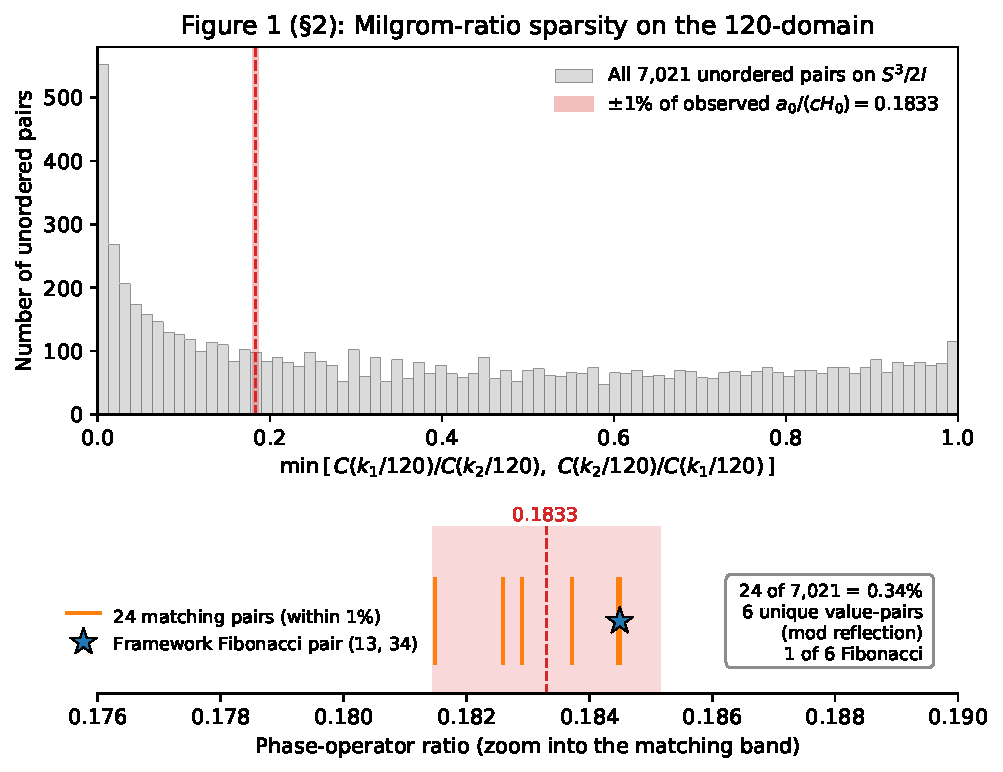
\includegraphics[width=\textwidth]{figures/figure1.pdf}
\caption{\label{fig:sparsity}Milgrom-ratio sparsity on the 120-domain.
Top: histogram of all 7,021 unordered phase-operator ratios on
$S^3/2I$, with vertical line at the observed Milgrom ratio
$a_0/(cH_0) = 0.1833$ and a shaded $\pm 1\%$ band marking the matching
region. Bottom: zoom into the band, with the 24 matching ratios as
orange ticks and the framework's $(13, 34)$ Fibonacci pair starred.
The 24 raw matches collapse to 6 unique phase-operator value-pairs
under the reflection symmetry $C(k) = C(120-k)$; the framework's
$(13, 34)$ pair is one of six in the Fibonacci subset
$\{13, 21, 34, 55\}/120$.}
\end{figure*}

% =====================================================================
\section{Five observable channels}
\label{sec:channels}
% =====================================================================

The evolution $a_0(z) = a_0(0)\,E(z)$ from Sec.~\ref{sec:derivation}
propagates into galactic observables through different powers of
$E(z)$. We adopt the flat $\Lambda$CDM Friedmann form
$E(z) = \sqrt{\Omega_m(1+z)^3 + \Omega_r(1+z)^4 + \Omega_\Lambda}$
with Planck 2018 parameters~\cite{Planck2018} ($\Omega_m = 0.315$,
$\Omega_r = 9.2 \times 10^{-5}$, $\Omega_\Lambda = 0.685$,
$H_0 = 67.4$~km/s/Mpc). The prediction $a_0(z) \propto H(z)$ holds for
any expansion history; adopting $\Lambda$CDM is a transparency choice
that allows direct comparison with published measurements.
Table~\ref{tab:cosmology} provides the reference values consumed by
the five channels below.

\begin{table}[tb]
\caption{\label{tab:cosmology}Predicted $a_0(z)$ and deep-MOND
enhancement factor across the redshift range relevant to this paper.}
\begin{ruledtabular}
\begin{tabular}{rrrrrr}
$z$ & $E(z)$ & $H(z)$~[km/s/Mpc] & $a_0(z)$~[m/s$^2$]
    & $\sqrt{E(z)}$ & $t_\text{age}$~[Gyr] \\
\hline
0.0  & 1.000  & 67.4   & $1.20 \times 10^{-10}$ & 1.000 & 13.79 \\
0.5  & 1.322  & 89.1   & $1.59 \times 10^{-10}$ & 1.150 & 8.58  \\
1.0  & 1.791  & 120.7  & $2.15 \times 10^{-10}$ & 1.338 & 5.84  \\
2.0  & 3.033  & 204.4  & $3.64 \times 10^{-10}$ & 1.741 & 3.27  \\
3.0  & 4.568  & 307.9  & $5.48 \times 10^{-10}$ & 2.137 & 2.14  \\
5.0  & 8.297  & 559.2  & $9.96 \times 10^{-10}$ & 2.880 & 1.17  \\
10.0 & 20.53  & 1383   & $2.46 \times 10^{-9}$  & 4.530 & 0.470 \\
15.0 & 36.01  & 2427   & $4.32 \times 10^{-9}$  & 6.001 & 0.268 \\
\end{tabular}
\end{ruledtabular}
\end{table}

\subsection{Tully-Fisher normalization: $E(z)^{-1}$}
\label{sec:btfr}

In the deep-MOND limit, the baryonic Tully-Fisher relation (BTFR) is
$v_\text{flat}^4 = G\,M_b\,a_0$~\cite{Lelli2016}. With evolving $a_0$:
\begin{equation}
\boxed{\;\frac{A_\text{BTFR}(z)}{A_\text{BTFR}(0)}
       = \frac{1}{E(z)}\;},
\qquad A_\text{BTFR} \equiv \frac{1}{G\,a_0}.
\label{eq:btfr-shift}
\end{equation}
The interpolating-function dependence cancels in the ratio: any
$\mu(x)$ that fits the local SPARC sample inherits the same fractional
evolution. At fixed baryonic mass,
$v_\text{flat}(z) = v_\text{flat}(0)\,E(z)^{1/4}$; at fixed velocity,
$M_b(z) = M_b(0)/E(z)$.

\begin{table}[tb]
\caption{\label{tab:btfr}BTFR evolution at six reference redshifts.}
\begin{ruledtabular}
\begin{tabular}{rrrr}
$z$ & $E(z)$ & $A(z)/A(0)$
    & $v_\text{flat}(z)/v_\text{flat}(0)$ at fixed $M_b$ \\
\hline
0.0  & 1.000  & 1.000 & 1.000 \\
0.5  & 1.322  & 0.756 & 1.072 \\
1.0  & 1.791  & 0.558 & 1.157 \\
2.0  & 3.033  & 0.330 & 1.320 \\
5.0  & 8.297  & 0.121 & 1.697 \\
10.0 & 20.53  & 0.049 & 2.128 \\
\end{tabular}
\end{ruledtabular}
\end{table}

An $L^*$ disk ($M_b = 6 \times 10^{10}\,M_\odot$,
$v_\text{flat}(0) = 176$~km/s) is predicted to have
$v_\text{flat}(z=2) = 232$~km/s, a 32\% increase at fixed baryonic
mass. The existing \"Ubler et al.~\cite{Ubler2017} KMOS3D measurement
is the only quantitative test of this prediction; the comparison is
treated in Sec.~\ref{sec:constraints}.

\subsection{MOND transition radius and asymptotic velocity:
$E(z)^{-1/2}$, $E(z)^{+1/4}$}
\label{sec:rotation}

The radius where Newtonian gravity equals $a_0(z)$ is
$r_M = \sqrt{G M_b / a_0(z)}$, giving
\begin{equation}
\boxed{\;\frac{r_M(z)}{r_M(0)} = \frac{1}{\sqrt{E(z)}}\;}.
\label{eq:rM-ratio}
\end{equation}
At $z = 2$, the transition happens at 57\% of the local radius. The
asymptotic velocity rises as $E(z)^{1/4}$ (from
Sec.~\ref{sec:btfr}). Both scalings are mass-independent in the
deep-MOND limit.

\begin{table*}[tb]
\caption{\label{tab:archetypes}Predicted MOND radius and asymptotic
velocity at $z = 0$ and $z = 2$ for four SPARC archetypes. The
fractional shifts $r_M(2)/r_M(0) = 0.574$ and
$v_\text{flat}(2)/v_\text{flat}(0) = 1.320$ apply identically across
the table.}
\begin{ruledtabular}
\begin{tabular}{lrrrrr}
Archetype & $M_b$~[$M_\odot$]
  & $r_M(0)$~[kpc] & $r_M(2)$~[kpc]
  & $v_\text{flat}(0)$~[km/s] & $v_\text{flat}(2)$~[km/s] \\
\hline
Dwarf (DDO 154)         & $3.5 \times 10^{8}$  & 0.64  & 0.37 & 49  & 64  \\
Sub-$L^*$ (NGC 2403)    & $1.0 \times 10^{10}$ & 3.41  & 1.96 & 112 & 148 \\
$L^*$ (NGC 6946)        & $6.0 \times 10^{10}$ & 8.35  & 4.79 & 176 & 232 \\
Giant (UGC 2885)        & $1.5 \times 10^{11}$ & 13.20 & 7.58 & 221 & 292 \\
\end{tabular}
\end{ruledtabular}
\end{table*}

The comparison isolates the effect of $a_0(z)$ at fixed baryonic
distribution. Real galaxies at $z = 2$ differ in structural
properties; the observer-facing formulation is: given an observed
galaxy at redshift $z$ with measured $M_b$ and
$v_\text{flat}^{\text{obs}}$, compare
$v_\text{flat}^{\text{obs}}/E(z)^{1/4}$ to the local SPARC value for
galaxies of the same $M_b$.

\subsection{Lensing dynamical mass: $E(z)^{+1/2}$}
\label{sec:lensing}

Galaxy-galaxy weak lensing infers a dynamical mass
$M_\text{dyn}(R) = v_\text{flat}^2 R / G$ within aperture $R$ under
the standard Newtonian inversion. This is a proxy-level prediction for
the mass that would be quoted under the standard Newtonian dynamical
inversion. It does not supply a relativistic lensing completion;
rather, it defines the redshift scaling that the framework predicts
for the Newtonian-equivalent $M_\text{dyn}$ reported by lensing
analyses. In the deep-MOND limit:
\begin{equation}
\boxed{\;\frac{M_\text{dyn}(R,z)/M_b}{M_\text{dyn}(R,0)/M_b}
        = \sqrt{E(z)}\;}.
\label{eq:lensing-shift}
\end{equation}
The enhancement is mass-independent and aperture-independent (for
$R \gg r_M$). At $z = 2$, $M_\text{dyn}/M_b$ is 74\% higher than at
$z = 0$ at any fixed mass and aperture (Fig.~\ref{fig:lensing}).

\begin{table}[tb]
\caption{\label{tab:lensing}Predicted $M_\text{dyn}/M_b$ for the
$L^*$ archetype at three lensing apertures.}
\begin{ruledtabular}
\begin{tabular}{rrrrrr}
$R$~[kpc] & $z=0$ & $z=0.5$ & $z=1$ & $z=2$ & $z=5$ \\
\hline
30  & 3.59  & 4.13  & 4.81  & 6.26  & 10.35  \\
100 & 11.98 & 13.77 & 16.03 & 20.86 & 34.50  \\
300 & 35.93 & 41.32 & 48.08 & 62.57 & 103.50 \\
\end{tabular}
\end{ruledtabular}
\end{table}

% Figure 2 (lensing discriminator) -- first cited at end of §3.3
\begin{figure*}[tb]
\centering
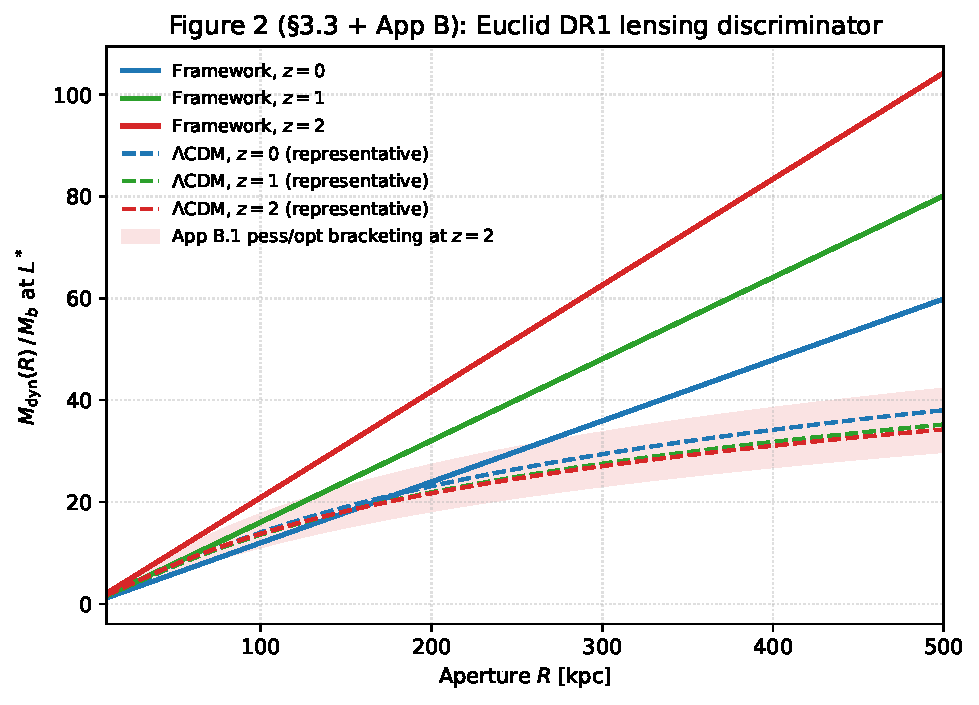
\includegraphics[width=\textwidth]{figures/figure2.pdf}
\caption{\label{fig:lensing}Euclid DR1 lensing discriminator. $L^*$
archetype $M_\text{dyn}(R)/M_b$ vs aperture $R$ at $z = 0, 1, 2$. The
framework prediction (solid curves) is the universal $\sqrt{E(z)}$
shift. The $\Lambda$CDM prediction (dashed curves) uses the $L^*$
NFW + Moster SHMR + Duffy concentration parameterization
(Appendix~\ref{app:lensing}); the shaded band at $z = 2$ shows the
pessimistic-to-optimistic bracketing under SHMR + concentration
variations from Table~\ref{tab:bracketing}. Even under generous
$\Lambda$CDM assumptions, the framework's $z = 2$ value sits well
above the upper bracket.}
\end{figure*}

Under $\Lambda$CDM, halo concentration evolution produces
$M_\text{dyn}/M_b$ shifts that depend on both mass and
aperture~\cite{Moster2013, Duffy2008}. The framework predicts a
universal $\sqrt{E(z)}$ factor across all masses and apertures. A
Euclid DR1 stacked analysis stratified by both galaxy stellar mass
and aperture tests the magnitude and the universality of the
prediction in a single dataset (Sec.~\ref{sec:euclid}).

\subsection{Collapse time: $E(z)^{-1/4}$ (supporting evidence)}
\label{sec:collapse}

In the deep-MOND regime, $g_\text{eff} = \sqrt{g_N \cdot a_0(z)}$
scales as $\sqrt{E(z)}$ at fixed source, and the free-fall time
$t_\text{ff} \propto 1/\sqrt{g_\text{eff}}$ shortens as
$E(z)^{-1/4}$. At $z \sim 8$, the factor $E(z)^{1/4} \approx 2$
shortens the characteristic deep-MOND collapse time by approximately
a factor of two. This eases, but does not by itself resolve, the
star-formation-efficiency pressure for the Labb\'e et
al.~\cite{Labbe2023} massive candidates. Whether this resolves the
impossibility constraint for any specific candidate depends on
halo-mass priors the framework does not modify; the per-object
analysis is reserved for future work. The fourth-root dependence
makes this channel robust: a 10\% shift in $E(z)$ changes the
correction by less than 3\%.

\subsection{Summary: five exponents from one input}
\label{sec:summary}

\begin{table*}[tb]
\caption{\label{tab:summary}The full predictive content of the
evolving acceleration scale, evaluated at $z = 2$.}
\begin{ruledtabular}
\begin{tabular}{lcrl}
Observable & Scaling & Value at $z = 2$ & Primary test \\
\hline
BTFR normalization                         & $E(z)^{-1}$
  & 0.330 & Euclid DR1, KMOS3D \\
MOND radius                                & $E(z)^{-1/2}$
  & 0.574 & High-$z$ rotation curves \\
Asymptotic velocity at fixed $M_b$         & $E(z)^{+1/4}$
  & 1.320 & Euclid DR1, KMOS3D \\
Lensing $M_\text{dyn}/M_b$                 & $E(z)^{+1/2}$
  & 1.741 & Euclid DR1 stacked lensing \\
Free-fall collapse time                    & $E(z)^{-1/4}$
  & 0.758 & JWST spectroscopy \\
\end{tabular}
\end{ruledtabular}
\end{table*}

The five exponents are correlated manifestations of one input
(Fig.~\ref{fig:exponents}). A measurement of any one observable at
any one redshift tests $a_0(z) = a_0(0)\,E(z)$ through that channel;
consistency across channels at the same $z$ tests the universality of
the deep-MOND scaling across observable classes.

% Figure 3 (five exponents) -- first cited end of §3.5
\begin{figure}[tb]
\centering
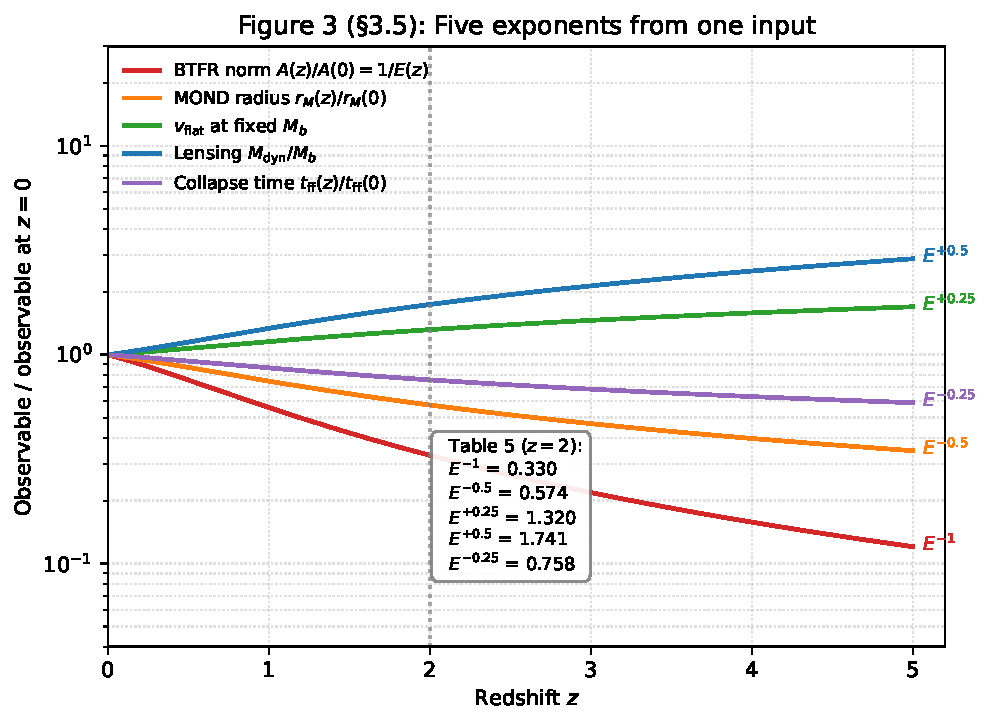
\includegraphics[width=\columnwidth]{figures/figure3.pdf}
\caption{\label{fig:exponents}Five exponents from one input.
Normalized observables $X(z)/X(0)$ vs redshift on log-y axes for the
five channels: BTFR normalization $1/E(z)$, MOND radius
$1/\sqrt{E(z)}$, asymptotic velocity at fixed $M_b$ as $E(z)^{1/4}$,
lensing $M_\text{dyn}/M_b$ as $\sqrt{E(z)}$, and free-fall collapse
time $E(z)^{-1/4}$. All curves emanate from $X(0) = 1$ and fan apart
with redshift; values at $z = 2$ are annotated and match
Table~\ref{tab:summary}.}
\end{figure}

% =====================================================================
\section{Existing constraints}
\label{sec:constraints}
% =====================================================================

\subsection{The \"Ubler tension}
\label{sec:ubler}

The KMOS3D analysis of \"Ubler et al.~\cite{Ubler2017} is the only
existing quantitative test of the Sec.~\ref{sec:btfr} prediction at
intermediate redshift. Their fixed-slope BTFR zero-point offsets
relative to the local Lelli et al.~\cite{Lelli2016} baseline are
\begin{equation*}
\Delta b^{\text{obs}}(z{=}0.9) = -0.44 \pm 0.04~\text{dex},
\quad \Delta b^{\text{obs}}(z{=}2.3) = -0.27 \pm 0.05~\text{dex}.
\end{equation*}
The framework predicts
\begin{equation*}
\Delta b^{\text{MIT}}(z{=}0.9) = -0.227~\text{dex},
\quad \Delta b^{\text{MIT}}(z{=}2.3) = -0.540~\text{dex}.
\end{equation*}
Two features matter. First, the magnitudes overlap: both the
prediction and the data place the high-$z$ BTFR substantially below
the local relation. Second, the trend shapes disagree: the data are
non-monotonic ($-0.44 \to -0.27$), while the prediction is strictly
monotonic ($-0.227 \to -0.540$) (Fig.~\ref{fig:ubler}).

% Figure 4 (Übler tension) -- first cited end of §4.1 first paragraph
\begin{figure}[tb]
\centering
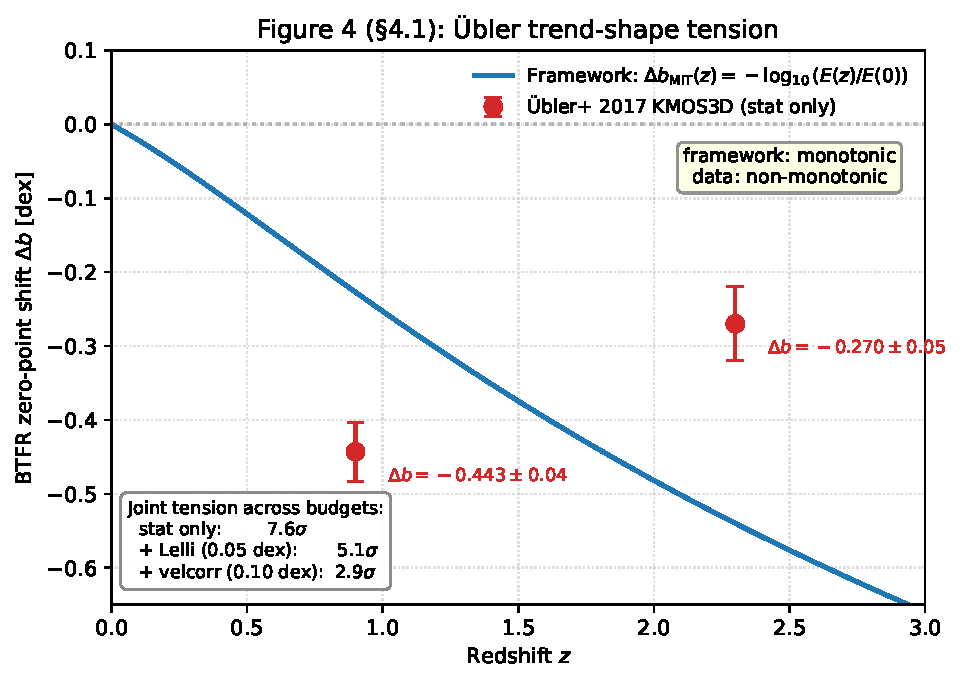
\includegraphics[width=\columnwidth]{figures/figure4.pdf}
\caption{\label{fig:ubler}\"Ubler trend-shape tension. BTFR
zero-point shift $\Delta b$ vs redshift. The framework prediction
(solid curve) is $-\log_{10}(E(z))$ under the anchored convention,
monotonically decreasing with no free parameter. The \"Ubler 2017
KMOS3D points (filled circles, statistical error bars) at $z = 0.9$
and $z = 2.3$ show a non-monotonic pattern incompatible with the
monotonic prediction. The joint tension across three uncertainty
budgets ranges from 7.6$\sigma$ (statistical only) to 2.9$\sigma$
(with 0.05 dex local-baseline + 0.10 dex velocity-correction
systematics).}
\end{figure}

The tension is quantified across three uncertainty budgets:

\begin{table}[tb]
\caption{\label{tab:tension}\"Ubler-tension table at three uncertainty
budgets: statistical only; with 0.05 dex local-baseline systematic;
with additional 0.10 dex velocity-correction systematic. Joint
tension is the quadrature combination across the two redshift bins.}
\begin{ruledtabular}
\begin{tabular}{lrrr}
Budget & $T(z=0.9)$~[$\sigma$] & $T(z=2.3)$~[$\sigma$]
       & Joint~[$\sigma$] \\
\hline
\"Ubler statistical only        & $-5.4$ & $+5.4$ & 7.6 \\
$+$ local-baseline (0.05 dex)   & $-3.4$ & $+3.8$ & 5.1 \\
$+$ velocity-correction (0.10 dex) & $-1.8$ & $+2.2$ & 2.9 \\
\end{tabular}
\end{ruledtabular}
\end{table}

Even under the most conservative budget, the joint tension is
2.9$\sigma$. We treat this as a provisional tension rather than a
formal falsification, because the comparison combines heterogeneous
velocity definitions and cross-redshift pressure-support
corrections. Formal falsification requires a matched-systematics
measurement: single instrument, uniform tracer, identical correction
prescription across redshift bins (Sec.~\ref{sec:euclid}).

We tested whether the \"Ubler radial pressure-support correction can
produce the observed non-monotonic pattern from a monotonic
underlying BTFR. Mock galaxies at $z = 0.9$ and $z = 2.3$ were
generated under the framework's prediction with literature-realistic
distributions of baryonic mass, scale length, and velocity
dispersion~\cite{Wisnioski2015}. The \"Ubler thick-disk correction
$v_\text{circ}^2(r) = v_\text{rot}^2(r) + 2\sigma_0^2\,r/R_d$ was
applied with the published selection cut
$v_\text{rot,max}/\sigma_0 > 4.4$. Four bias models (radial-position
uncertainty, beam-smearing of $\sigma_0$, non-asymptotic rotation
curves, selection-induced mass shifts) were swept over
literature-plausible ranges. None reproduces the observed
$(-0.44, -0.27)$ pattern. The closest combined model recovers
$(-0.295, -0.472)$, leaving the $z = 0.9$ point 0.15 dex above
observed. The mock-generation script, parameter ranges, and random
seeds will be deposited with the supplementary material.

The tension is genuine and not a velocity-correction artifact. The
prediction stands. Resolution will come from Euclid DR1
matched-tracer kinematics and JWST follow-up at the original \"Ubler
redshifts (Sec.~\ref{sec:euclid}).

\subsection{Galaxy clusters}
\label{sec:clusters}

MOND analyses of local galaxy clusters~\cite{PointecouteauSilk2005}
report a residual mass discrepancy of roughly a factor of 5 at
$r \approx 0.5\,R_\text{vir}$. The framework's evolving $a_0$ does
not address this: the relevant clusters sit at $z \lesssim 0.15$,
where $E(z) \leq 1.08$ and the framework correction is less than
8\%. A factor-of-5 problem is not touched by an 8\% correction. This
discrepancy is an open problem shared by all MOND-class
theories~\cite{Sanders2003, Angus2008, Famaey2012} and predates the
present framework, which neither introduces nor resolves it.

\subsection{The CMB at recombination}
\label{sec:cmb}

A naive application of $a_0(z)$ to cosmological perturbations at
$z = 1090$ gives $a_0 \approx 23{,}000 \times a_0(0)$, placing
recombination-scale perturbations deep in the MOND regime and
disrupting the acoustic peak structure that Planck fits at
sub-percent precision.

The framework's selection rule (Sec.~\ref{sec:derivation},
Appendix~\ref{app:framework-selection}) separates this channel
structurally. The rule assigns $a_0$ to the edge sector ($n = 1$,
$\Omega_H$) and cosmological perturbations to the space sector
($n = 3$, $\Omega_\Lambda$). Under this assignment, the $a_0(z)$
scaling governs galactic dynamics and does not propagate to
perturbation evolution. The same rule independently produces the
Sec.~\ref{sec:derivation} Milgrom-ratio match at 0.7\% and the
$\Lambda$-constant prediction; it was not introduced to address the
CMB.

The consistency condition is quantitative. Writing a minimal leakage
coupling $g_\text{eff} = g_N + \varepsilon\sqrt{g_N\,a_0(z)}$, the
Planck first-peak amplitude (0.5\% tolerance) constrains
$\varepsilon \leq 1.2 \times 10^{-5}$. The framework predicts
$\varepsilon = 0$ under exact edge/space decoupling, satisfying the
bound by five orders of magnitude. A first-principles
perturbation-theory derivation of the decoupling is flagged as the
principal open task for the framework's CMB-scale predictions
(Appendix~\ref{app:framework-open}).

\subsection{Other regimes}
\label{sec:other}

Local SPARC and THINGS measurements are consistent by construction:
the well assignments were calibrated against $a_0(0)$ and $H_0$ at
$z = 0$ (Sec.~\ref{sec:derivation}). The Genzel et
al.~\cite{Genzel2017} SINS/zC-SINF sample of six massive
star-forming disks at $z = 0.9\text{--}2.4$ reports declining outer
rotation curves with low inferred dark-matter fractions; because no
fixed-slope BTFR zero-point is published, the data are qualitatively
consistent with Sec.~\ref{sec:btfr} but do not provide a
quantitative test of the normalization prediction. Strong-lensing
time-delay cosmography (TDCOSMO~\cite{Millon2020},
H0LiCOW~\cite{Wong2020}) is below current sensitivity to the
framework's predictions. None of these regimes is sharp enough to
test the framework's normalization prediction independently.

\subsection{Summary}
\label{sec:constraints-summary}

\begin{table}[tb]
\caption{\label{tab:constraints}Constraint status across five
regimes.}
\begin{ruledtabular}
\begin{tabular}{ll}
Regime & Status \\
\hline
Local ($z = 0$)
  & Consistent by construction \\
Intermediate-$z$ BTFR (\"Ubler~\cite{Ubler2017})
  & Provisional 2.9$\sigma$ tension on trend shape \\
Galaxy clusters~\cite{PointecouteauSilk2005}
  & Inherited, unaddressed ($\sim 8\%$ vs factor-5) \\
CMB ($z = 1090$)
  & Structurally decoupled; $\varepsilon \leq 1.2 \times 10^{-5}$ from Planck \\
Strong-lens time delays
  & Below current sensitivity \\
\end{tabular}
\end{ruledtabular}
\end{table}

One live tension, one inherited problem, one structural decoupling,
two consistencies. The \"Ubler tension is held against the prediction
without retreat.

% =====================================================================
\section{The Euclid DR1 test}
\label{sec:euclid}
% =====================================================================

Euclid's stated objective is to characterize the dark Universe and
its evolution across $z = 0\text{--}2$~\cite{Mellier2024}. The
framework gives two structurally inverse predictions in that sector:
$a_0(z) \propto H(z)$ in galactic dynamics (this paper); $\Lambda$
constant (companion paper). The Euclid DR1 release in October 2026
is expected to deliver the sharpest test of the $a_0(z)$ prediction
through stacked galaxy-galaxy weak lensing at $z = 0.5\text{--}2$.

\paragraph*{What Euclid measures.}
The wide survey is expected to provide the photometric redshifts,
stellar-mass estimates, galaxy shapes, and sample sizes needed for a
stacked galaxy-galaxy lensing test. For the framework, the relevant
observable is the Newtonian-equivalent $M_\text{dyn}/M_b$ inferred
from stacked tangential shear profiles after mass and redshift
stratification. Equation~(\ref{eq:lensing-shift}) is a prediction for
this quoted proxy, not a standalone relativistic lensing law. The
Sec.~\ref{sec:euclid} test is accordingly a test of the proxy-level
prediction, not of a relativistic lensing theory the framework does
not yet supply.

\paragraph*{What the framework predicts.}
At fixed baryonic mass and aperture, $M_\text{dyn}/M_b$ is enhanced
by $\sqrt{E(z)}$ relative to $z = 0$: a 15\% excess at $z = 0.5$,
34\% at $z = 1$, and 74\% at $z = 2$ (Table~\ref{tab:lensing}). The
enhancement is universal across galaxy mass and lensing aperture in
the deep-MOND regime.

\paragraph*{Why this discriminates from $\Lambda$CDM.}
Under $\Lambda$CDM, $M_\text{dyn}/M_b$ also evolves with redshift
through halo concentration evolution and stellar-to-halo mass
relation shifts~\cite{Moster2013, Duffy2008}. The $\Lambda$CDM
prediction is mass-dependent and aperture-dependent: at $z = 2$
relative to $z = 0$, the $\Lambda$CDM ratio shifts by a factor of
0.76 for a Sub-$L^*$ galaxy, 0.98 for $L^*$, and 1.13 for a Giant at
the canonical $R = 100$~kpc aperture, spanning 37 percentage points
across the mass range (Appendix~\ref{app:lensing}). The framework
predicts the same factor 1.74 for all three. A Euclid DR1 analysis
stratified by both stellar mass and aperture tests the magnitude and
the universality of the prediction in a single dataset.

\paragraph*{Falsification criteria.}

\begin{table*}[tb]
\caption{\label{tab:falsification}Falsification criteria for the five
Sec.~\ref{sec:channels} predictions. A matched-systematics
discrepancy at $\geq 2\sigma$ is treated as a reportable tension;
formal falsification requires either $\geq 3\sigma$ in one channel
or mutually consistent $\geq 2\sigma$ failures across independent
redshift bins or observables.}
\begin{ruledtabular}
\begin{tabular}{p{0.18\textwidth}p{0.30\textwidth}p{0.27\textwidth}p{0.18\textwidth}}
Prediction & Signature & Reportable tension if & Key systematic \\
\hline
BTFR normalization
  & $A(z)/A(0) = 1/E(z)$
  & Single-$z$ inconsistency at $\geq 2\sigma$
  & Pressure-support correction \\
BTFR trend shape
  & Monotonic decrease
  & Non-monotonic trend confirmed under matched systematics
  & Cross-instrument tracer mismatch \\
MOND radius
  & $r_M(z)/r_M(0) = E(z)^{-1/2}$
  & Single-$z$ inconsistency at $\geq 2\sigma$
  & Baryonic mass model \\
Lensing enhancement
  & $\sqrt{E(z)}$, mass/aperture-independent
  & Inconsistency at $\geq 2\sigma$, or mass/aperture-dependent shift
  & Halo concentration evolution \\
Collapse-time correction
  & $t_\text{ff}(z)/t_\text{ff}(0) = E(z)^{-1/4}$
  & Corrected formation timescales incompatible with spectroscopic
    ages at $\geq 2\sigma$
  & Halo-mass priors \\
\end{tabular}
\end{ruledtabular}
\end{table*}

The lensing row is the cleanest because $\sqrt{E(z)}$ is universal
while the $\Lambda$CDM alternative is not. A mass- and
aperture-stratified Euclid analysis tests both the magnitude of the
prediction and its universality simultaneously.

\begin{table*}[tb]
\caption{\label{tab:schedule}Near-term test schedule.}
\begin{ruledtabular}
\begin{tabular}{p{0.30\textwidth}p{0.27\textwidth}p{0.25\textwidth}p{0.13\textwidth}}
Window & Instrument & Tests & Delivery \\
\hline
Stacked lensing, $z = 0.5\text{--}2$
  & Euclid DR1
  & Lensing enhancement, universality
  & October 2026 \\
Emission-line sample selection
  & Euclid NISP grism
  & Lens sample definition, redshift binning
  & October 2026 \\
Matched-tracer BTFR
  & JWST NIRSpec IFU / ground IFU
  & BTFR normalization, trend shape
  & In progress \\
Resolved kinematics at \"Ubler redshifts
  & JWST NIRSpec IFU
  & BTFR at $z = 0.9$, $z = 2.3$
  & In progress \\
Spectroscopic confirmation, $z = 7\text{--}9$
  & JWST NIRSpec
  & JWST efficiency
  & 2025--2026 \\
\end{tabular}
\end{ruledtabular}
\end{table*}

All programs listed are existing or imminent. No new instrument or
observational capability is required. This paper and its predictions
are deposited on Zenodo (concept DOI:
\href{https://doi.org/10.5281/zenodo.19980665}{10.5281/zenodo.19980665})
prior to the Euclid DR1 release, fixing the numbers before the data
arrive.

% =====================================================================
\section{Conclusions}
\label{sec:conclusions}
% =====================================================================

The Milgrom coincidence $a_0 \approx cH_0$ resolves, within the
bounded-topology framework of Appendix~\ref{app:framework}, to a
fixed ratio of two phase-operator values at adjacent Fibonacci wells:
$a_0/(cH) = C(13/120)/C(34/120) = 0.1845$, agreeing with the observed
$0.1833$ at $0.7\%$. The $a_0$ and $H$ wells are fixed by separately
calibrated assignments at $z = 0$ sharing the same edge-mode
hierarchy; the ratio follows algebraically and is unique among the
framework's Fibonacci-well pairs (Sec.~\ref{sec:derivation}).

Because both observables reference the same epoch-dependent
hierarchy, the ratio holds at every cosmic epoch:
$a_0(z) = a_0(0)\,E(z)$. Five observable channels follow as different
powers of $E(z)$, with no additional free parameter. The BTFR
normalization shifts as $E(z)^{-1}$, the MOND transition radius
contracts as $E(z)^{-1/2}$, the asymptotic velocity at fixed baryonic
mass rises as $E(z)^{+1/4}$, the lensing-inferred dynamical mass
enhancement scales as $E(z)^{+1/2}$, and the gravitational collapse
time shortens as $E(z)^{-1/4}$. The five exponents are correlated,
not independent: consistency across channels at the same redshift
tests the universality of the deep-MOND scaling.

The prediction lives in a constraint landscape with one genuine
tension (\"Ubler et al.\ KMOS3D BTFR trend shape at 2.9$\sigma$,
tested by forward modeling and not dissolved), one inherited problem
(cluster-scale MOND discrepancy, untouched by the framework's
$\lesssim 8\%$ low-redshift correction), and one structural
decoupling (CMB via the selection rule, with leakage bounded to
$\varepsilon \leq 1.2 \times 10^{-5}$ by Planck). The \"Ubler
tension is acknowledged and held against the prediction without
retreat.

A companion analysis (separately submitted) makes the structurally
inverse prediction from the same scaling law: $\Lambda$ remains
constant, and the apparent $w(z)$ evolution reported by DESI DR2 is a
template artifact. The two predictions test different sectors of the
framework's selection rule through disjoint instruments.

The sharpest scheduled test is Euclid DR1 in October 2026: stacked
galaxy-galaxy lensing at $z = 0.5\text{--}2$ stratified by mass and
aperture, probing both the predicted 74\% enhancement and its
universality in a regime where the framework and $\Lambda$CDM
produce quantitatively distinct shifts. This paper and its
predictions are deposited on Zenodo (concept DOI:
\href{https://doi.org/10.5281/zenodo.19980665}{10.5281/zenodo.19980665})
prior to that release.

% =====================================================================
\begin{acknowledgments}
% =====================================================================

The author thanks the observational teams whose published data made
this work possible: the SPARC collaboration (Lelli, McGaugh,
Schombert) for the local rotation-curve sample~\cite{Lelli2016,
McGaugh2016RAR}; \"Ubler and the KMOS3D team for the
intermediate-redshift Tully-Fisher measurements~\cite{Ubler2017};
Wisnioski and the KMOS3D team for the kinematic-dispersion data used
in the Sec.~\ref{sec:ubler} forward model~\cite{Wisnioski2015};
Genzel and the SINS/zC-SINF team for the high-redshift rotation
curves~\cite{Genzel2017}; Pointecouteau and Silk for the X-ray
cluster analysis~\cite{PointecouteauSilk2005}; the JWST observing
teams and the Labb\'e group for the early-galaxy
catalog~\cite{Labbe2023}; the Planck collaboration for the
cosmological parameters and CMB amplitudes~\cite{Planck2018}; and
the DESI collaboration for the dark-energy survey
results~\cite{DESI2025}. No external funding supported this work.

\end{acknowledgments}

% =====================================================================
\section*{Data availability}
% =====================================================================

All numerical predictions, tabulated framework outputs, and source
code for the analysis pipelines and figure-generation scripts are
archived at Zenodo (concept DOI:
\href{https://doi.org/10.5281/zenodo.19980665}{10.5281/zenodo.19980665}),
mirrored from \url{https://github.com/dmobius3/a0z} (release v1.1.0).
The archive includes the combinatorial baseline table (supporting
Sec.~\ref{sec:derivation}); the Sec.~\ref{sec:channels}--%
\ref{sec:euclid} prediction tables (Tables~\ref{tab:cosmology}--%
\ref{tab:summary}) in CSV format; the $\Lambda$CDM lensing
discriminator overlay (NFW enclosed-mass curves at the canonical
archetypes, supporting Sec.~\ref{sec:lensing} and
Appendix~\ref{app:lensing}); the \"Ubler $\sigma$-tension table
(supporting Sec.~\ref{sec:ubler}); the CMB leakage-bound table
(supporting Sec.~\ref{sec:cmb}); and the Labb\'e candidate speedup
factors (supporting Sec.~\ref{sec:collapse}).

% =====================================================================
\appendix

\section{Framework foundations}
\label{app:framework}
% =====================================================================

This appendix supplies the structural detail behind the
Sec.~\ref{sec:derivation} derivation. The bounded topology, phase
operator, scaling law, and selection rule are stated in
Sec.~\ref{sec:derivation}. This appendix develops the 120-domain
(\ref{app:framework-domain}), the selection rule's physical basis
(\ref{app:framework-selection}), the well-assignment eligibility
conditions (\ref{app:framework-wells}), the local-epoch reading in
full (\ref{app:framework-localepoch}), and the framework-level open
items (\ref{app:framework-open}).

\subsection{The 120-domain}
\label{app:framework-domain}

The physical observable space is the quotient $S^3/2I$, where $2I$
is the binary icosahedral group with $|2I| = 120$. The discrete
subgroups of $\text{SU}(2) \cong S^3$ are classified: cyclic groups
$\mathbb{Z}_n$, binary dihedral groups $2D_n$, and three exceptional
groups (binary tetrahedral $|2T| = 24$, binary octahedral
$|2O| = 48$, binary icosahedral $|2I| = 120$). Two constraints
select $2I$.

First, $2I$ is the largest exceptional discrete subgroup of
$\text{SU}(2)$, giving the maximum spectral resolution compatible
with $S^3$. In the framework, the quotient order $|2I| = 120$
defines the discrete phase domain used to label observable
positions, with spacing $\Delta\Theta = 1/120$.

Second, the icosahedron is the unique Platonic solid whose branch
orders $(2, 3, 5)$ are consecutive Fibonacci numbers satisfying
$2 + 3 = 5$. This Fibonacci-recurrence structure makes the
Fibonacci positions on the 120-domain the natural stable lattice
(Appendix~\ref{app:framework-selection} below and the Hurwitz
stability argument in Appendix~\ref{app:framework-wells}).

The phase position is quantized:
$\Theta \in \{k/120 : k = 0, 1, \ldots, 119\}$. For photon-mediated
observables, the bosonic projection $|\psi|^2$ erases the
anti-periodic sign flip, halving the resolution to a 60-position
grid (even numerators only). The framework implements this as a
bosonic projection: photon-mediated observables sample the
60-position quotient, while dynamical observables may access the
full 120-domain.

The chronon, the smallest phase advance the domain can register, is
$\Delta t_\text{min} = 4\pi/120 = \pi/30$, giving a minimum action
$\Delta S_\text{min} = \hbar\pi/30$ that is frame-independent by
construction.

\subsection{The selection rule}
\label{app:framework-selection}

The scaling law (Sec.~\ref{sec:derivation},
Eq.~\ref{eq:scaling-law}) assigns each observable a manifold-mode
index $n$ from the embedding hierarchy
$S^1 \subset \text{M\"obius} \subset S^3$ and a corresponding
hierarchy normalization $N$. The physical basis for the
$(n, \Omega)$ assignment is:

\paragraph*{Edge modes ($n = 1$, $\Omega_H$).}
The boundary $S^1$ is a kinematic locus: it carries no intrinsic
eigenvalue (the surface eigenvalue lives one dimension up, on the
M\"obius strip, where $\Lambda$ is placed). What an edge-mode
observable references is the embedding scale of $S^1$ in the ambient
cosmological geometry. The natural such scale is the Hubble horizon
$R_H = c/H$, and its dimensionless Planck ratio is
$\Omega_H \approx (c/(H\ell_P))^2$. Because $H$ evolves with cosmic
epoch, edge-mode observables inherit that evolution through the
calibrated normalization $N_H(z) = H(z)\,t_P/C(34/120)$.

\paragraph*{Surface modes ($n = 2$, $\Omega_\Lambda$).}
The M\"obius strip carries an intrinsic eigenvalue: the ground mode
of the Laplace-Beltrami operator on the totally geodesic surface in
$S^3$ gives $\lambda_0 = 2/R^2$, where $R$ is the curvature radius
of $S^3$. The Gauss-Codazzi embedding converts this to
$\Lambda_\text{obs} = (3/2)\lambda_0 = 3/R^2$ under three
conditions: totally geodesic embedding ($K_{ij} = 0$), isotropy
(CMB-verified to $10^{-5}$), and de Sitter vacuum. The hierarchy
ratio $\Omega_\Lambda = (\Lambda\ell_P^2)^{-1}$ is set by this
eigenvalue and does not evolve.

\paragraph*{Space modes ($n = 3$, $\Omega_\Lambda$).}
Cosmological perturbations propagate on the spatial slice $S^3$ and
reference the same fixed eigenvalue hierarchy as the surface. Under
this assignment, perturbation evolution is governed by
$\Omega_\Lambda$, not $\Omega_H$, and inherits no $a_0(z)$
modification. This is the structural basis for the CMB consistency
argument in Sec.~\ref{sec:cmb}.

The selection rule is a postulate of the framework, not derived
from the topology. Its empirical support is the set of percent-level
agreements it produces: $\Lambda$ at 2\%, $\alpha$ at 0.5\%, and the
Milgrom ratio at 0.7\%, across observables spanning 122 orders of
magnitude from a single rule.

\subsection{Well assignments}
\label{app:framework-wells}

Three eligibility conditions determine which Fibonacci wells are
consistent with each observable:

\begin{enumerate}
\item \textbf{Manifold index} separates edge modes ($n = 1$: $H_0$,
$a_0$) from surface modes ($n = 2$: $\Lambda$).

\item \textbf{Bosonic projection.} Photon-mediated observables
access only the 60-grid (even numerators); dynamical observables
access the full 120-grid.

\item \textbf{Antinode requirement.} $\Lambda$, as a topologically
protected eigenvalue, sits at $\Theta = 60/120$ where
$d\ln C/d\Theta = 0$.
\end{enumerate}

The Fibonacci wells on the 120-domain are
$\{13, 21, 34, 55\}/120$, corresponding to $F_7$ through $F_{10}$.
The lower bound $F_7 = 13$ is the noise floor: below this, the
amplitude $C(k/120)$ is indistinguishable from neighboring positions.
The upper bound $F_{10} = 55$ is set by the reflection symmetry
$C(k) = C(120 - k)$, which makes $F_{11} = 89$ equivalent to
$F_8 = 21$. These bounds are motivated by the Hurwitz stability
criterion: $\varphi$ is the irrational hardest to approximate by
rationals of bounded denominator, so Fibonacci positions on the
120-domain are taken to minimize destructive interference between
modes.

Under the eligibility conditions:

\begin{enumerate}[label=(\alph*)]
\item $a_0$ is assigned $\Theta = 13/120$: the unique coprime
position ($\gcd(13, 120) = 1$), accessible only on the full 120-grid
as required for a dynamical (non-photon-mediated) observable.

\item $H_0$ is assigned $\Theta = 34/120$: the unique even-numerator
Fibonacci well among $\{13, 21, 34, 55\}/120$, consistent with the
bosonic-projection condition for a photon-mediated observation.

\item $\Lambda$ is assigned $\Theta = 60/120$: the antinode, where
the phase operator takes its maximum and the log-slope vanishes.
\end{enumerate}

The wells $21/120$ and $55/120$ remain unassigned in this paper. The
assignments have the status of empirical calibrations at $z = 0$
that land on positions compatible with the eligibility conditions.
The manifold-mode classification, bosonic-projection filter,
selection rule, and the prediction $a_0(z) \propto H(z)$ were
established in the framework's foundational
deposit~\cite{ShattoMIT2025} prior to the present paper's
calibration, foreclosing post-hoc adjustment of the eligibility
conditions to fit the well assignments. A first-principles
derivation from the Hurwitz/Fibonacci structure of the 120-domain
is future work.

\subsection{The local-epoch reading}
\label{app:framework-localepoch}

The body Sec.~\ref{sec:derivation} states the local-epoch reading
in one paragraph. Here is the full argument.

Three components of the scaling law (Eq.~\ref{eq:scaling-law}) are
topological and do not evolve: the phase operator $C(\Theta)$ is
fixed by the 120-domain (Appendix~\ref{app:framework-domain}), the
manifold index $n$ is fixed by the embedding hierarchy, and the
Fibonacci wells are fixed by Hurwitz stability
(Appendix~\ref{app:framework-wells}). The sole evolving component
is the hierarchy normalization $N_H(z)$, calibrated through the
local Hubble rate $H(z)$ at the observer's epoch via
Eq.~(\ref{eq:H-calibration}).

The local-epoch reading says: a measurement performed at epoch $z$
calibrates $N_H$ through the local $H(z)$, not through some
privileged past or future value. This is the default reading of a
measurement postulate: it specifies what an observer measures at
the measurement event.

The alternative would anchor $N_H$ permanently to its present-day
value $N_H(0)$, so that all edge-mode observables retain their
$z = 0$ values at every epoch. Under this alternative, $a_0$ is
constant. But this alternative requires introducing an external
preferred epoch into the scaling law. The bounded domain $S^3$ with
$\partial S^3 = \emptyset$ has no preferred time slice: the
standing wave $\Psi(t) = \cos(t/2)$ is $t$-dependent throughout, and
the framework refuses to fix a privileged epoch anywhere in the
cycle.

The local-epoch reading is therefore not a separate postulate added
to the framework. It is the refusal to add one. Freezing $N_H(0)$
would be the addition; the local reading is the default.

Observable distinguishability: the two readings ($a_0$ evolves vs
$a_0$ constant) produce quantitatively different predictions at
every $z > 0$. At $z = 2$, the BTFR normalization differs by a
factor of 3 between the two readings. The Euclid DR1 test
(Sec.~\ref{sec:euclid}) will distinguish them.

\subsection{Open items}
\label{app:framework-open}

Two framework-level open questions are flagged for completeness:

\begin{enumerate}
\item \textbf{CMB perturbation-theory derivation.} The edge/space-mode
decoupling (Appendix~\ref{app:framework-selection}) is a structural
argument supported by the Planck leakage bound
$\varepsilon \leq 1.2 \times 10^{-5}$ (Sec.~\ref{sec:cmb}). A
first-principles derivation from the Boltzmann hierarchy under the
framework's $(n, \Omega)$ assignments would replace the structural
argument with a closed-form proof. The required machinery
(mode-projected propagators, anti-periodic boundary conditions,
hierarchy-sensitive transfer functions) is expressible within the
framework's existing postulates; the calculation has not been
carried through.

\item \textbf{Well-position derivation.} The well assignments
(Appendix~\ref{app:framework-wells}) are empirical calibrations at
$z = 0$. A derivation of the assignments from the
Hurwitz/Fibonacci structure of the 120-domain, independent of the
$z = 0$ measurements, would elevate the well positions from
calibrated inputs to derived outputs. This is the next foundational
step after the present prediction paper.
\end{enumerate}

Neither open item affects the
Sec.~\ref{sec:channels}--\ref{sec:euclid} predictions or the
Sec.~\ref{sec:euclid} falsification criteria; both are flagged as
future work within the framework's existing postulate set.

% =====================================================================
\section{$\Lambda$CDM lensing comparison methodology}
\label{app:lensing}
% =====================================================================

Section~\ref{sec:lensing} and Sec.~\ref{sec:euclid} compare the
framework's universal $\sqrt{E(z)}$ lensing enhancement against the
$\Lambda$CDM prediction under halo concentration evolution. This
appendix specifies the parameterization.

\subsection{Galaxy archetypes and halo parameters}
\label{app:lensing-archetypes}

Four baryonic-mass archetypes span the SPARC range:

\begin{table}[h]
\caption{\label{tab:archetypes-app}Four baryonic-mass archetypes
spanning the SPARC range.}
\begin{ruledtabular}
\begin{tabular}{lr}
Archetype & $M_b$~[$M_\odot$] \\
\hline
Dwarf (DDO 154)         & $3.5 \times 10^{8}$  \\
Sub-$L^*$ (NGC 2403)    & $1.0 \times 10^{10}$ \\
$L^*$ (NGC 6946)        & $6.0 \times 10^{10}$ \\
Giant (UGC 2885)        & $1.5 \times 10^{11}$ \\
\end{tabular}
\end{ruledtabular}
\end{table}

Representative halo masses and concentrations at the $L^*$
archetype, consistent with Moster et al.~\cite{Moster2013}
stellar-to-halo mass relation and Duffy et al.~\cite{Duffy2008}
concentration evolution:

\begin{table}[h]
\caption{\label{tab:halo}Representative $(M_\text{halo}, c)$ at the
$L^*$ archetype across three reference redshifts.}
\begin{ruledtabular}
\begin{tabular}{rrr}
$z$ & $M_\text{halo}$~[$M_\odot$] & $c$ \\
\hline
0 & $1.5 \times 10^{12}$ & 7.5 \\
1 & $1.0 \times 10^{12}$ & 5.0 \\
2 & $7.0 \times 10^{11}$ & 3.5 \\
\end{tabular}
\end{ruledtabular}
\end{table}

Sub-$L^*$ and Giant archetypes use mass-appropriate
$(M_\text{halo}, c)$ values from the same parameterization. The
SHMR mapping is used only to set representative halo masses; the
discriminator depends on the relative mass- and aperture-dependence
of the $\Lambda$CDM prediction, not the absolute baryonic-to-halo
normalization. These are representative defaults; alternative SHMR
inversions shift the absolute $\Lambda$CDM values but preserve the
mass- and aperture-dependence that constitutes the
Sec.~\ref{sec:euclid} discriminator.

\subsection{NFW enclosed mass}
\label{app:lensing-nfw}

The dynamical mass at fixed physical aperture $R$ is
\begin{equation*}
M_\text{dyn}(R, z) = M_\text{NFW}(R; M_\text{halo}, c, z) + M_b,
\end{equation*}
with NFW enclosed mass
\begin{equation*}
M_\text{NFW}(R) = M_\text{halo} \cdot
\frac{\ln(1 + R/r_s) - (R/r_s)/(1 + R/r_s)}
     {\ln(1 + c) - c/(1 + c)},
\end{equation*}
scale radius $r_s = R_\text{vir}/c$, and virial radius under the
$R_{200}$ convention:
\begin{equation*}
R_\text{vir}^3 = \frac{3\,M_\text{halo}}
                       {4\pi \cdot 200 \cdot \rho_\text{crit}(0)\,E(z)^2}.
\end{equation*}
The ratio $M_\text{dyn}/M_b$ is computed under the same Newtonian
inversion used by the framework prediction
(Sec.~\ref{sec:lensing}, Eq.~\ref{eq:lensing-shift}).

\subsection{The discriminator}
\label{app:lensing-discriminator}

At the canonical $R = 100$~kpc aperture, the $\Lambda$CDM
$M_\text{dyn}/M_b$ ratio at $z = 2$ relative to $z = 0$ is:

\begin{table}[h]
\caption{\label{tab:lcdm-mass}$\Lambda$CDM $M_\text{dyn}/M_b$
ratio $z=2/z=0$ at $R = 100$~kpc across three baryonic-mass
archetypes, against the framework's universal prediction.}
\begin{ruledtabular}
\begin{tabular}{lrr}
Archetype & $\Lambda$CDM ratio ($z{=}2/z{=}0$) & Framework ratio \\
\hline
Sub-$L^*$ & 0.76 & 1.74 \\
$L^*$     & 0.98 & 1.74 \\
Giant     & 1.13 & 1.74 \\
\end{tabular}
\end{ruledtabular}
\end{table}

The $\Lambda$CDM prediction spans 37 percentage points across the
mass range (0.76 to 1.13); the framework predicts a universal
1.74. At fixed $L^*$ mass, the $\Lambda$CDM ratio also varies with
aperture: 1.07 at $R = 30$~kpc, 0.98 at $R = 100$~kpc, 0.92 at
$R = 300$~kpc; the framework predicts 1.74 at all three.

\paragraph*{Sensitivity bracketing.}
Table~\ref{tab:bracketing} evaluates the same NFW pipeline under
pessimistic and optimistic SHMR + concentration parameterizations at
the $L^*$ archetype, $R = 100$~kpc.

\begin{table*}[tb]
\caption{\label{tab:bracketing}$\Lambda$CDM $L^*$ $M_\text{dyn}/M_b$
at $R = 100$~kpc under three parameterizations, against the
framework's universal prediction.}
\begin{ruledtabular}
\begin{tabular}{lcccc}
Parameterization
  & $(M_\text{halo}, c)$ at $z = 0$
  & $(M_\text{halo}, c)$ at $z = 2$
  & $M_\text{dyn}/M_b$: $z{=}0$ / $z{=}2$
  & Framework / $\Lambda$CDM at $z{=}2$ \\
\hline
Pessimistic
  & $(2.0 \times 10^{12}, 9.0)$
  & $(1.0 \times 10^{12}, 4.5)$
  & 17.7 / 17.5
  & 1.19 \\
Representative
  & $(1.5 \times 10^{12}, 7.5)$
  & $(7.0 \times 10^{11}, 3.5)$
  & 14.0 / 13.8
  & 1.52 \\
Optimistic
  & $(1.0 \times 10^{12}, 6.0)$
  & $(5.0 \times 10^{11}, 2.5)$
  & 10.3 / 11.2
  & 1.86 \\
\textbf{Framework (universal)}
  & ---
  & ---
  & \textbf{11.98 / 20.86}
  & --- \\
\end{tabular}
\end{ruledtabular}
\end{table*}

Even under the pessimistic parameterization, the framework's
$z = 2$ prediction sits 19\% above the $\Lambda$CDM upper bracket.
The normalized evolution-ratio framing
($1.74/0.98 \simeq 1.78$) inherits this robustness with additional
cancellation, since the $\Lambda$CDM $z = 2$ and $z = 0$ endpoints
shift correlatedly under SHMR and concentration variations and the
ratio is more stable than either absolute value.

A Euclid DR1 stacked analysis stratified by both stellar mass and
aperture tests the framework on two axes simultaneously: the
magnitude of the redshift shift and its universality across mass
and aperture. In normalized redshift evolution at $L^*$, the
discriminator is $1.74/0.98 \simeq 1.78$, well above the
statistical scale expected for large stacked samples, though the
limiting uncertainty will be systematic calibration rather than raw
shape noise.

Cosmological parameters: Planck 2018~\cite{Planck2018},
$\rho_\text{crit}(0) = 8.53 \times 10^{-27}$~kg/m$^3$,
$\Omega_m = 0.315$, $\Omega_\Lambda = 0.685$,
$H_0 = 67.4$~km/s/Mpc.

% =====================================================================
\begin{thebibliography}{22}
% =====================================================================

\bibitem{Milgrom1983}
M. Milgrom, Astrophys.\ J.\ \textbf{270}, 365 (1983).

\bibitem{Lelli2016}
F. Lelli, S. S. McGaugh, and J. M. Schombert,
Astron.\ J.\ \textbf{152}, 157 (2016).

\bibitem{Famaey2012}
B. Famaey and S. S. McGaugh,
Living Rev.\ Relativ.\ \textbf{15}, 10 (2012).

\bibitem{Milgrom1999}
M. Milgrom, Phys.\ Lett.\ A \textbf{253}, 273 (1999).

\bibitem{McGaugh2004}
S. S. McGaugh, Astrophys.\ J.\ \textbf{611}, 26 (2004).

\bibitem{Planck2018}
Planck Collaboration VI,
Astron.\ Astrophys.\ \textbf{641}, A6 (2020).

\bibitem{Labbe2023}
I. Labb\'e \emph{et al.}, Nature \textbf{616}, 266 (2023).

\bibitem{BoylanKolchin2023}
M. Boylan-Kolchin,
Nat.\ Astron.\ \textbf{7}, 731 (2023).

\bibitem{DESI2025}
DESI Collaboration, arXiv:2503.14738 (2025).

\bibitem{Ubler2017}
H. \"Ubler \emph{et al.}, Astrophys.\ J.\ \textbf{842}, 121 (2017).

\bibitem{Moster2013}
B. P. Moster, T. Naab, and S. D. M. White,
Mon.\ Not.\ R.\ Astron.\ Soc.\ \textbf{428}, 3121 (2013).

\bibitem{Duffy2008}
A. R. Duffy, J. Schaye, S. T. Kay, and C. Dalla Vecchia,
Mon.\ Not.\ R.\ Astron.\ Soc.\ \textbf{390}, L64 (2008).

\bibitem{Wisnioski2015}
E. Wisnioski \emph{et al.},
Astrophys.\ J.\ \textbf{799}, 209 (2015).

\bibitem{PointecouteauSilk2005}
E. Pointecouteau and J. Silk,
Mon.\ Not.\ R.\ Astron.\ Soc.\ \textbf{364}, 654 (2005).

\bibitem{Sanders2003}
R. H. Sanders,
Mon.\ Not.\ R.\ Astron.\ Soc.\ \textbf{342}, 901 (2003).

\bibitem{Angus2008}
G. W. Angus, B. Famaey, and D. A. Buote,
Mon.\ Not.\ R.\ Astron.\ Soc.\ \textbf{387}, 1470 (2008).

\bibitem{Millon2020}
M. Millon \emph{et al.},
Astron.\ Astrophys.\ \textbf{639}, A101 (2020).

\bibitem{Wong2020}
K. C. Wong \emph{et al.},
Mon.\ Not.\ R.\ Astron.\ Soc.\ \textbf{498}, 1420 (2020).

\bibitem{Mellier2024}
Euclid Collaboration: Y. Mellier \emph{et al.},
arXiv:2405.13491 (2024).

\bibitem{ShattoMIT2025}
B. Shatto, \emph{Mode Identity Theory: Modal Realization from
Nested Topology} (2025),
\href{https://doi.org/10.5281/zenodo.18064856}{DOI:10.5281/zenodo.18064856}.

\bibitem{McGaugh2016RAR}
S. S. McGaugh, F. Lelli, and J. M. Schombert,
Phys.\ Rev.\ Lett.\ \textbf{117}, 201101 (2016).

\bibitem{Genzel2017}
R. Genzel \emph{et al.}, Nature \textbf{543}, 397 (2017).

\end{thebibliography}

\end{document}
